\documentclass[tikz]{standalone}

\begin{document}
\begin{minipage}{0.25\linewidth}
    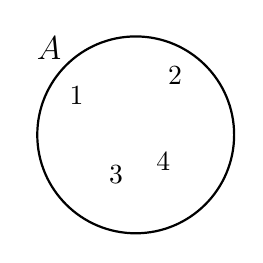
\begin{tikzpicture}
        \draw[thick] (0,0) circle[radius=1.25];
        \draw (-0.75,0.5) node{$1$}
            (0.5,0.75) node{$2$}
            (-0.25,-0.5) node{$3$}
            (0.35,-0.34) node{$4$}
            (-1.1,1.1) node{\large $A$};
    \end{tikzpicture}
\end{minipage}\hspace{40pt}
\begin{minipage}{0.25\linewidth}
    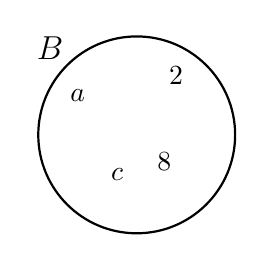
\begin{tikzpicture}
        \draw[thick] (0,0) circle[radius=1.25];
        \draw (-0.75,0.5) node{$a$}
            (0.5,0.75) node{$2$}
            (-0.25,-0.5) node{$c$}
            (0.35,-0.34) node{$8$}
            (-1.1,1.1) node{\large $B$};
    \end{tikzpicture}
\end{minipage}
\end{document}
